Generell besteht der verwendete Aufbau aus drei Teilen, welche nachfolgend genauer beschrieben werden.
Damit die Datenaufnahme am Rechner reibungslos funktioniert muss der Aufbau in der richtigen Reihenfolge erfolgen.
Das generelle Schema ist in Abbildung \ref{fig:aufbau} dargestellt.

\begin{figure}
  \centering
  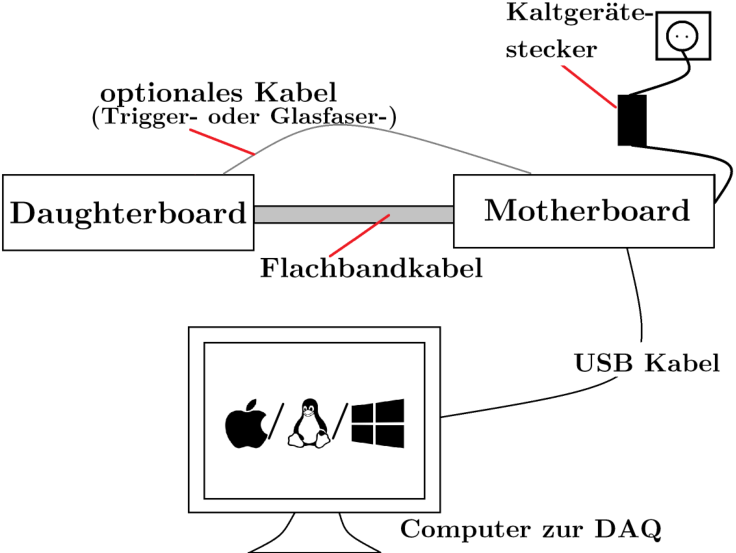
\includegraphics[width=0.5\textwidth]{content/graphics/aufbau.png}
  \caption{Aufbau und Verkabelung des benutzten Detektorsystems.}
  \label{fig:aufbau}
\end{figure}

Zunächst wird die Detektor- mit der Kontrolleinheit über ein Flachbandkabel verbunden.
Dieses dient der Spannungsversorgung des Detektors und überträgt die aufgenommenen Daten und Steuersignale.
Für die Quellenmessung wird weiterhin ein Triggerkabel verbunden und für die Messung mittels Laserlicht wird ein Glasfaserkabel genutzt.
Danach wird die Kontrolleinheit per USB an den Rechner angeschlossen.
Erst danach wird die Kontrolleinheit mit Strom versorgt.
Danach ist das mitgelieferte Programm zu starten und es sollte lediglich eine grüne LED an der Kontrolleinheit leuchten.
Soll eine Quellenmessung durchgeführt werden, so ist die Detektoreinheit in eine mit Bleisteinen verkleideten Kiste zu legen.
Das oben erwähnte Triggerkabel ist anzuschließen und der Schieber der Detektoreinheit in die Q-Position zu schieben.
Anschließend wird die Quelle platziert.
Für Messungen mit dem Laser befindet sich der Reiter in der L-Position.

\subsection{Detektoreinheit}

Die Detektoreinheit beherbergt den eigentlichen Siliziumstreifendetektor und die zugehörige Auseleseelektronik.
Wie in Abschnitt \ref{sec:theorie} kurz angedeutet, entspricht der Aufbau des Chips denen des ATLAS-Detektors und ist in 128 Streifen aufgeteilt, die jeweils $\SI{10}{\micro\metre}$ voneinander entfernt sind.
Die Signale der einzelnen Streifen werden durch den BEETLE Chip ausgelesen, welcher über Wirebonds mit ihnen verbunden ist.
Damit größtenteils nur echte Signale aufgenommen werden, wartet der BEETLE Chip auf ein Signal des Triggers bevor die Daten tatsächlich an die Kontrolleinheit gesendet werden.
Die Kontrolleinheit digitalisiert das Signal und wandelt es in ADC Counts um.
Damit die Messung erfolgreich durchgeführt werden kann, muss der Detektor vollständig deplettiert sein.
Die zugehörige Depletionsspannung wird auf einen Bereich von $U_{dep} = 60$ bis $\SI{80}{\volt}$ vom Hersteller angegeben.
Dies soll später verifiziert werden.
Oberhalb des Detektors befindet sich eine verschiebbare Plattform, die das Lasersystem und ein Carbonplättchen trägt.
Das Carbonplättchen ist undurchlässig für Licht, aber durchlässig für ionisierende Strahlen, was es optimal für Messungen mit radioaktiven Quellen macht.
Das Lasersystem kann über Millimeterschrauben mit einer Präzision von $$\SI{10}{\micro\metre}$$ kalibriert werden.
Die horizontale Millimeterschraube verschiebt den Laser in horizontaler Richtung und ermöglicht die Positioniereung des Lasers über verschiedenen Streifen.
Zur Fokussierung kann die vertikale Schraube verwendet werden.
Erzeugt wird der Laser dabei nicht innerhalb des Lasersystems auf der Detektoreinheit, sondern in der Kontrolleinheit und muss deswegen mittels eines Glasfaserkabels zunächst mit der Einheit verbunden werden.
Die Wellenlänge des Lasers beträgt $\SI{980}{\nano\metre}$, der Durchmesser $\SI{20}{\micro\metre}$ und die Spitzenleistung $\SI{0.6}{\milli\watt}$ bei einer Pulslänge von $\SI{5}{\nano\second}$.
Das Aussehen der Detektoreinheit ist in Abbildung \ref{fig:detektoreinheit} zu sehen.

\begin{figure}
  \centering
  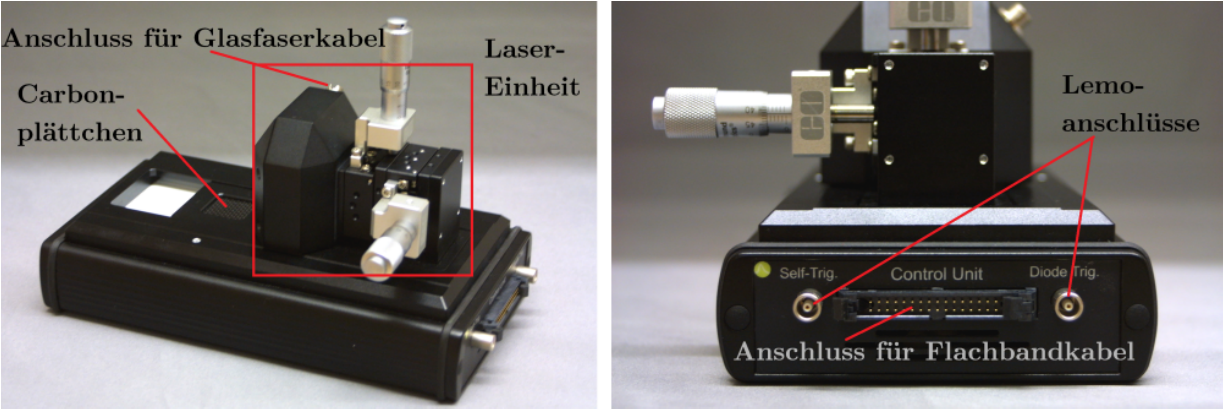
\includegraphics[width=0.8\textwidth]{content/graphics/detektoreinheit.png}
  \caption{Die verwendete Detektoreinheit in Aufsicht und Frontalansicht.}
  \label{fig:detektoreinheit}
\end{figure}

\subsection{Der Halbleitersensor}

In der Detektoreinheit ist ein Halbleiterdetektor aus Silizium verbaut.
Die Basis bildet eine $\SI{300}{\micro\metre}$ dicke n-dotierte Siliziumschicht auf der 128 p-dotierte Siliziumstreifen aufgebracht sind.
Es handelt sich somit um einen p-in-n Sensor.
Diese Streifen sind gegeneinder durch eine Siliziumoxidschicht isoliert.
Dies ermöglicht die Lokalisierung der deponierten Ladung und verhindert ein direktes Fließen des Leckstroms in die Ausleseelektronik.
Eine Aluminiumschicht dient als Elektrode.
Diese ist durch die Siliziumoxidschicht von den Streifen getrennt und ist daher nur kapazitiv mit diesen gekoppelt.
Ein umlaufender Bias Ring dient als Spannungsversorgung der Streifen, wohingegen der Guard Ring ein unkontrolliertes abfließen der Ladungsträger aus dem Detektor verhindert.
Eine Schrägansicht des Detektors ist in Abbildung \ref{fig:schragansicht} dargestellt.
Damit eine genaue Messung der Energiedeposition möglich wird, muss der Detektor vollständig deplettiert sein.

Um ionisierende Strahlung vermessen zu können, verfügt der Detektor über eine Triggervorrichtung.
Diese soll verhindern, dass Ereignisse aufgenommen werden, die nicht von externer Strahlung herrührt.
Dafür befindet sich einige Millimeter unterhalb des Detektors eine Siliziumdiode.
Dies ist in Abbildung \ref{fig:trigger} dargestellt.
Nur Elektronen die durch den gesamten Detektor geflogen sind und Energie in der Diode deponieren können werden somit registriert.
Ein Signal der Triggerdiode gibt die im BEETLE Chip vorgehaltenen Signale frei.

Die Effizienz der Ladungssammlung (Charge Collection Efficiency, CCE) steigt mit der Dicke der Depletionszone an.
Sie kann durch den Leser mittels der Formel

\begin{equation}
  \label{eqn:Eindringtiefe}
  CCE(U) = \frac{1 - \exp(\frac{-d_c(U)}{a})}{1 - \exp(\frac{-D}{a})}
\end{equation}

berechnet werden.
Dabei bezeichnet $d_C$ die Dicke der Depletionszone, $D$ die Sensordicke = $\SI{300}{\micro\metre}$ und $a$ die mittlere Eindringtiefe des Lasers.
Diese liegt bei einer Wellenlänge von $\SI{980}{\nano\metre}$ bei $\SI{74}{\micro\metre}$.
Die Dicke der Depletionszone berechnet sich durch

\begin{align}
  \begin{split}
    d_c(U) &= D \sqrt{\frac{U}{U_{dep}}} \,\text{für}\, U < U_{dep} \\
    d_c(U) &= D  \,\text{für}\, U \geq U_{dep},
  \end{split}
\end{align}

mit der Depletionsspannung $U_{dep}$.


\begin{figure}
  \begin{subfigure}{0.45\textwidth}
    \centering
    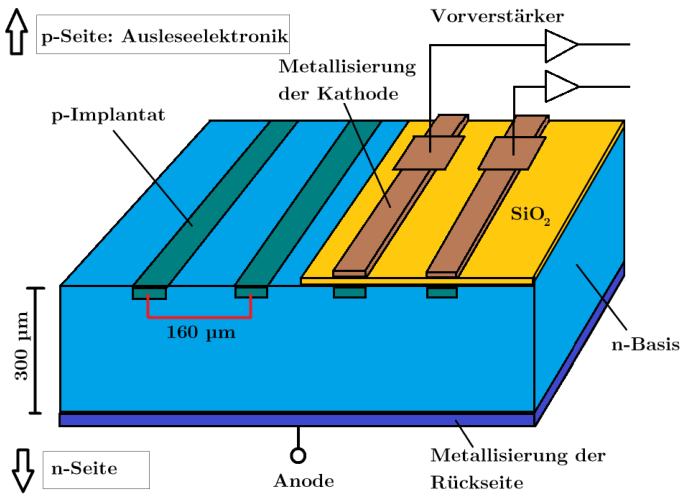
\includegraphics[width=\linewidth]{content/graphics/schrag.png}
    \caption{Schematisches Schrägansicht des verwendeten Siliziumstreifendetektors. Zu sehen sind die p-dotierten Streifen, die n-dotierte Basis, die Siliziumoxidschicht und die Kathode.}
    \label{fig:schragansicht}
  \end{subfigure}%
  \begin{subfigure}{0.45\textwidth}
    \centering
    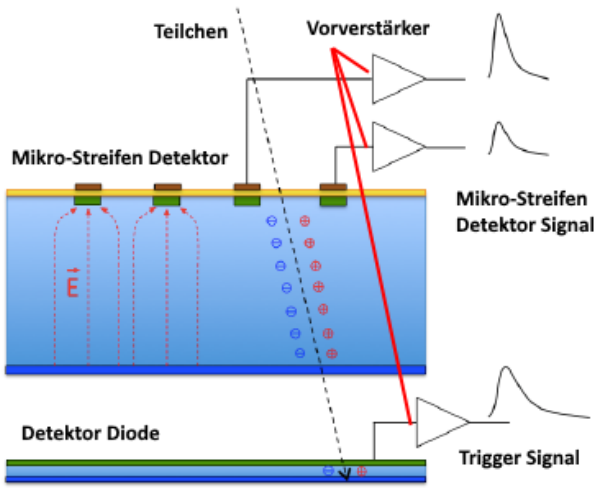
\includegraphics[width=\linewidth]{content/graphics/trig.png}
    \caption{Schematische Darstellung des Querschnitts durch den Siliziumstreifendetektor mit untergelagerter Triggerdiode. Eingezeichnet ist eine Teilchenspur, die durch den Detektor fliegt und Elektron-Loch Paare erzeugt. Da ein Signal ebenfalls im trigger erzeugt wird, wird dieses Signal aufgenommen.}
    \label{fig:trigger}
  \end{subfigure}%
  \caption{}
\end{figure}

\subsection{Störsignale}

Der Sensor und die Ausleseelektronik wie der BEETLE Chip erzeugen Störsignale, die die Messung negativ beeinflussen.
Sie verändern das eigentliche Signal und erschweren eine korrekte Auslesung.
Sie werden allumfassend als Rauschen, oder im Englischen Noise, bezeichnet.
Rauschen kann niemals gänzlich eliminiert werden, aber die Effekte können zumindest auf ein Minimum reduziert werden.
Der so tatsächlich gemessene ADC Count für ein Signal $k$ des Streifens $i$ besteht aus den folgenden Komponenten:

\begin{equation}
  \mathup{ADC}(i,k) = \mathup{P}(i,k) + \mathup{D}(k) + \mathup{Signal}(i,k).
\end{equation}

Dabei bezeichnet $\mathup{P}(i)$ das Pedestal des Streifens.
Das Pedestal ist der Mittelwert der ADC COunts eines Streifens ohne ein externes Signal $\mathup{Signal}(i,k)$.
Dieses Pedestal berechnet sich nach $N$ Messungen ohne Quelle zu

\begin{equation}
  \mathup{P}(i) = \frac{1}{N} \sum^N_{k=1} \mathup{ADC}(i,k).
\end{equation}

Weiterhin verfügt jeder der 128 Kanäle über einen Pedestal Offset von 500 ADC Counts.
Eine globale, alle Streifen betreffende Störung wird Common Mode Shift $\mathup{D}(k)$ genannt und berechnet sich durch

\begin{equation}
  \mathup{D}(k) = \frac{1}{128} \sum^{128}_{i=1} (\mathup{ADC}(i,k) - \mathup{P}(i)).
\end{equation}

Schlussendlich bestimmt sich die Noise jedes einzelnen STreifens durch den Root-Mean-Square der ADC Counts nachdem das Pedestal und der Common Mode Shift abgeszogen wurden.
Dies erfolgt nach der Gleichung

\begin{equation}
  \mathup{Noise}(i) = \sqrt{ \frac{1}{1 - N}  \sum^N_{k = 1} ( \mathup{ADC}(i,k) - \mathup{P}(i) - \mathup{D}(k))^2  }.
\end{equation}

Dieses Rauschen wird natürlich bei jeder Signalgenerierung mit aufgezeichnet und in die ADC Counts umgewandelt.
Relevante Signalereignisse sollen durch einen Signal-to-Noise-Cut vom Rauschen unterschieden werden.
Dabei wird das entstandene Signal durch das Rauschen des betreffenden Streifens geteilt.
Dieser Wert wird mit dem Cutwert verglichen.
Das Signal muss also ein Vielfaches (hier 5) des Rauschens betragen damit es weiter in der Analyse berücksichtigt wird.

Durch charge sharing und cross talk kann es zu der Bildung von Clustern kommen.
Cluster meint in diesem Fall, dass benachbarte Streifen das gleiche Signal sehen.
Charge Sharing bezeichnet den Vorgang, dass ein Teilchen am Rande eines Streifens herfliegt und seine Ladung auch im benachbarten Streifen deponiert.
Crosstalk hingegen meint, dass während der Auslesung das Signal des einen Streifens eine Signal in der Auslesekette des anderen Streifens induziert.
Und natürlich treten auch Teilchenspuren auf, die nicht nur durch einen Streifen fliegen, sondern durch mehrere da sie nicht senkrecht zur Oberfläche verlaufen.


















%
